\chapter{Implementation}\label{cha:implementation}

The following chapter will documet the different functional modules that were implemented according to the proposal. Most of them interact with each other through the SMs, which has been added as well as a module for its understanding.


\section{LED Control}\label{sec:leds}

The robot counts" with at least two LED rings that notify to the user the overall state of each access, this is considered only a visual aid which means that is not critical for the system. Currently there is a control for them using Arduino* devices. One of the goals of this prototype is to integrate the control of the LED rings within a single board; therefore, different apporaches were taken into account depending on the stages and experience in devloping on STM32 chips and its IDEs.
The following stages were carried out:
\subsection{Technical background}
*Here comes one picture of the LED ring and a very brief description of the LED and its interface, is it interface or protocol?-> interface*
Also a basic description of DMA in STM32

\subsection{Development*}
\begin{description}
\item[First control tests] Learning the basics of the interface used to control one LED
\item[Writing code for one LED control] Using the peripherals of the MCU, simple routines were written to set different basic colors in RGB. The peripherals used were a PWM channel and one timer to keep control of the timing.
\item[Exploration of libraries] Once the basic communication was understood, it was clear that the usage of libraries would be more practical since the control demanded cofnigurable number of LEDs and updating all of them at once, even with the possibility of including effects. From this exploration around STM32, the codes were mainly divided in two types: libraries for 8/16 bits processors that whose main task was controlling the LEDs, and a pair of libraries that used DMA Module within 32-bit processor. The latter was divided into two different approaches, namely rewritting an unique buffer for only one PWM channel and another highly focused on performance by divinding a circular buffer and interrupting the main processor only to update parts of it as the data was sent.
\item[First library selection] Due to the unexperience working with DMA modules and as the LED control was not of a high priority as the EtherCAT implementation, it was decided to run first one of the basic libraries to achieve a multi LED control and look for its adequating to the Axis Communication Board*.
\item[Trial of adequation of the library into the SM task] *here comes the explanation of why that library did not match with a multitask apporach*
\item[Second library selection] As the first library was able to control a set of 20 LEDs, some drawbacks were found in the approach, since the processor was focused only on polling Timers states. Event though, this first trial helped improving the overall understanding of the host MCU and the LEDs, it was not suitable to multi-tasking. Moreover, usage of DMA became clearer and it was decided to improve the approach by selecting a 32-bit processor based library. The Library* was then included and following the guidelines of the GNU* license it was modified to use two independant PWM generators -easily extendable* to four-. Furthermore, the main logic* of the library was divided such that its execution becomes non-sequential but triggered by events. The new interactions with other parts of the code can be seen in following subsections for SM*s.
\end{description}



\section{Temperature acquisition}\label{sec:temperature}

\subsection{Technical background}
*Here comes the image of the sensor, datasheet and summary of translating the one-wire protocol to usart*
\subsection{Development}
\begin{description}
\item[First readouts] Within the project's schedule this was the first set of test, so through them the IDE stm32cubei was learnt, along with the general configuration of the MCU. First trials* included set up of internal clocks, interruptions, GPIO basic usage, basic configuration of freeRTOS in STM32 *here comes a reference to a future subsection where the structure and relation of freeRTOS and CMSIS is explained*; as well as the introduction to the one-wire protocol. The first approach, similar to the one of the LED, was to understand the sensor and its protocol. Therefore, self written functions were tested based on peripherals, namely two timers, through which the timing of the data streams are controled as wel as the duration of ones and zeros. This approach worked as intended but it was knew from the beginning that does not match the multi-tasking and that further was needed. This implementation was able only to access in a generic way to the temperature conversion, and further functions were needed to access the sensor's ROM needed e.g. for identification.
\item[Readouts as a task/FreeRTOS first tests] Short after the working code was used to do the first tests with the RTOS, in this manner the code was translated as a Task (Thread as used by CMSIS) and some features like prioritization, task attributes, task handling and signals were tested with other generic functions, e.g. clocks and pwm generators or blinking LEDs. *here could come a reference to the captures of signals and PWM being generated and interrupted*. However, this implementation was not able to handle multiple one-wire devices due to its abscense of CRC** comparison.
\item[Integration of library] Finally, it was decided to adapt one open source library designed for STM32 processors. This is based on the principle that UART speeds @9600 and @11200 bps suits the One-Wire timing, such that the detection of One-Wire devices and communication process can be downloaded to hardware already included in many general-purposes processors using USART. The integration of this library is from design compatible with RTOS, namely with CMSIS-RTOS within the smt32cube development environment.
\end{description}


\section{Extra SPI Service/Auxiliar}\label{sec:spi}

An extra SPI apart from the one that is used to interface the MCU host to the LAN9252 Evaluation Board was included in the design, mainly for comming applications and development that may include interface SPI sensors, for instance, IMU sensors. The DMA streams and pins had to be taken into account to avoid overlapping functions** with other functionalities.
This section will also wrap the auxiliar functional block such that it can be addressed similarly to the proposed structure in Fig. ~\ref{fig:sysStruct}.

\section{EtherCAT Slave communication: SOES adaptation}\label{sec:soes}
This functional module is the one with highest priority, therefore most of the effort given was focused not only 
on the library itself but the protocol and the hardware commissioning. Hence, this section was extended and divided
as follows: first, more technical details are presented regarding the EtherCAT specification, such that the SOES
features are better understood. As to the next subsection, some constraints for the prototype are commented and the 
available hardware is explained*. Once summarized, the main points of the implementeation are presented.

\subsection{EtherCAT data consistency and constraints for design}\label{sec:ecat_sms}
This subsection describes both the features with which the \emph{Axis Communication Board} has compatibility, and a summary of the mechanism that the protocol
implements at the low level to work with the data exchange between Master and Slave. The constraints that were set were part of a live process that ran all along
the learning process of the protocol itself. This is important to mention, since the understanding of the protocol leads to a sinful selection of the features
that a device should have implemented. Therefore, the understing process was a natural consequence from the integration of the SOES library. It is presented however before, such that 
it is understandable what features became priorities and which others are now presented as proposals.

The reader may recall the set of Communication Profiles that are available within the EtherCAT fieldbus, see \ref{sec:ecat_protocol}. From them, the Mailbox and CoE 
are the main features with which the Axis Communication Board works. Leaving aside for future integration the FoE and EoE, the forme would make possible 
update the device by sending a firmware binaries to the device's bootloade; whereas the latter would make the ACB* accessible for any IT tool based on TCP/IP.

\begin{figure}[ht]
    \centering
    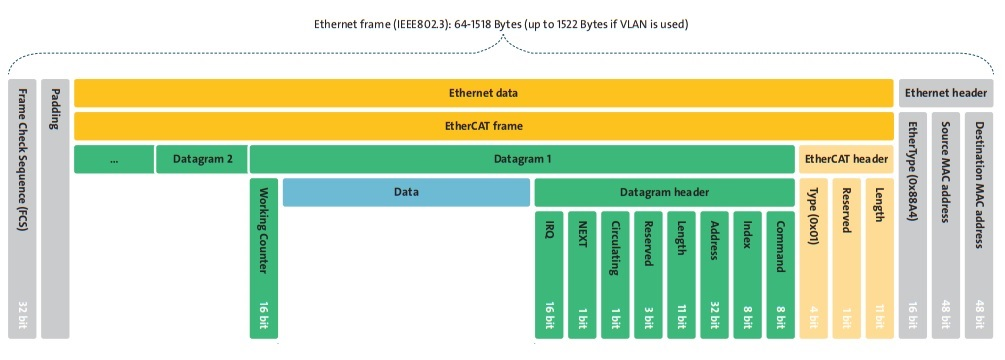
\includegraphics[width=\textwidth]{imgs/impl-dataframe.jpg}
    \caption{EtherCAT Datagram within the Ethernet Frame. Source: ETG.1000.4 - EtherCAT frame structure.}
    \label{fig:dataframe}
\end{figure}

\subsubsection{The data frame and the Synchronization Managers}
Besides the challange of setting up the hardware and basic firmware for a correct data transmission between ESC and the host MCU; the description of the EtherCAT 
Slave device is a task that demands, at least, a basic understanding of the data frame exchange and how the protocol demands its synchronization. From here on, the following
topics are going to be summarized: Synchronization modes and managers.
Whenever there are Real Time constraints, and the device takes part of a control loop, synchronization modes are needed to be set correctly between the Master and
any Device present. For this task the Distributed Clocs (DC) are need to be synchronzied. [?][?] %ETG.1020 - Synchronization and ETG.2000 - DC

There are three synchronization modes:  
\begin{description}
    \item[Free Run] Application is triggered by local clock and runs independently from EtherCAT cycle. 
    \item[SM-Synchronous] Application is synchronized whenever there are process data being written to the Synchronization Manager 2 (SM2).
    Moreover, any event generated by the Master is mapped onto an internal register or physically triggering an IRQ Pin of the ESC. 
    \item[DM-Synchronous] Within this synchronization mode the frame jitter can be even reduce down to $ns$ and use two different synchronization
    units within the ESC, namely the SM2 and SYNC/LATCH UNIT. 
\end{description}

The scope of this prototype covers the Freerun and SM-Synchronous mode, as they are the basic ones for communication Master-Slave. A graphical representation of them
is shown in figure \ref{fig:syncmodes}.

\begin{figure}[ht]
    \centering
    \subfigure[Free Run]{\label{subfig:syncm1}{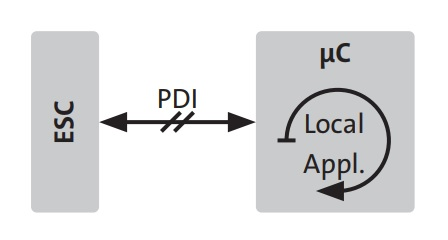
\includegraphics[width=0.3\textwidth]{imgs/impl-sync1.jpg}}}\hfill
    \subfigure[SM-Synchronization]{\label{subfig:syncm2}{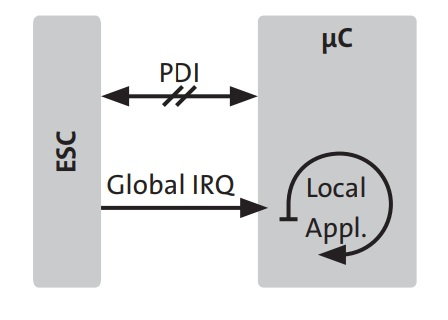
\includegraphics[width=0.3\textwidth]{imgs/impl-sync2.jpg}}}\hfill
    \subfigure[DC-Synchronization modes]{\label{subfig:syncm3}{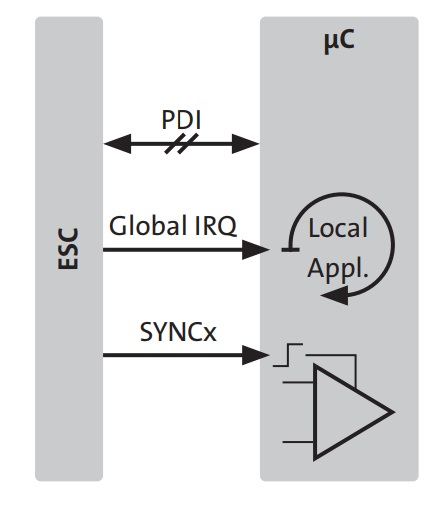
\includegraphics[width=0.3\textwidth]{imgs/impl-sync3.jpg}}}
    \caption{Synchronization modes defined in ETG.1000. Source [?]} %EtherCAT Device Protocol poster from EtherCAT resources
    \label{fig:syncmodes}
\end{figure} 

SMXs (Synchronization Managers 1,2,3 ...) coordinate access to the ESC memory from both sides, EtherCAT and
Host MCU (PDI). In case of process data communication it ensures that process data can
always be written to the memory by EtherCAT and can always be read by PDI side and vice versa (3-buffer mode). SyncManager 2/3 length is equal
to the Data Object lengths defined for receive and transmit data chunks respectively. [?] %ETG.1000.4 Sync manager
The mapping of the process data objects within the Ethernet Frame can be seen in figure \ref{fig:dataframe} and \ref{fig:pdomapping}.
The correct setup of the SMXs ensure the consistency of the data and needs to be linked correctly depending on the specifactions of each type of ESC,
 and SW Stack that are being used, this information is also linked to the CoE Object Dictionary (OD) and EtherCAT Slave Information (ESI) file.
\begin{figure}[ht]
    \centering
    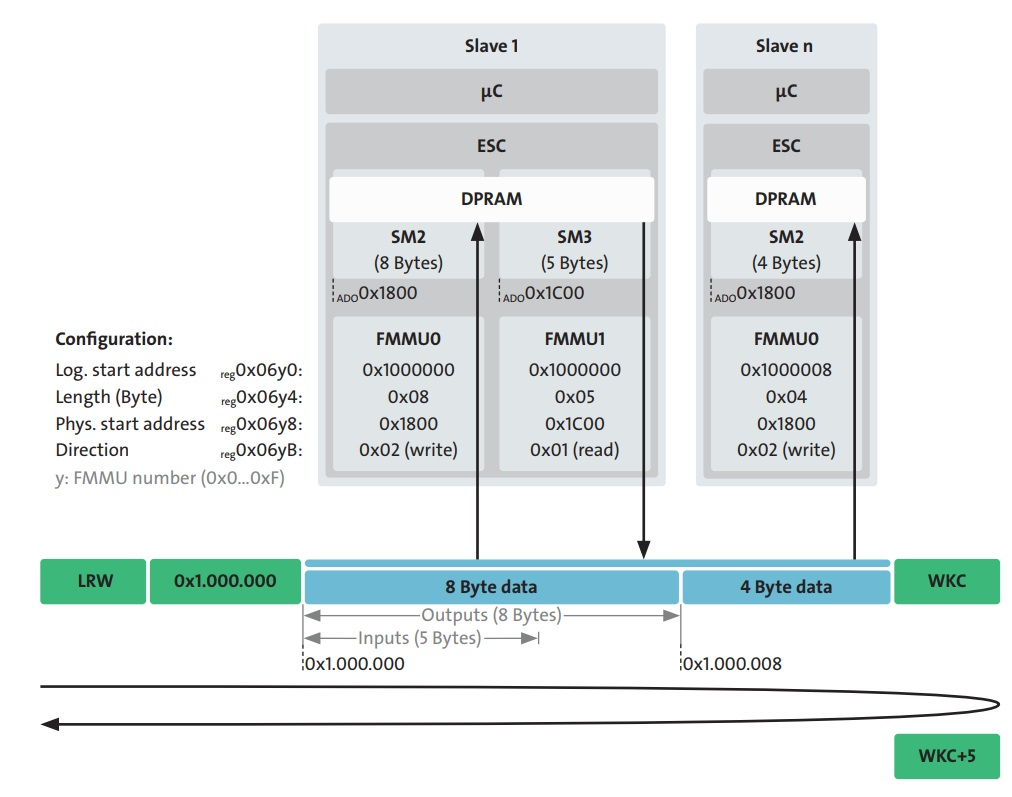
\includegraphics[width=.85\textwidth]{imgs/impl-dataframe_pdo.jpg}
    \caption{Depending on the different states of the Slave, there will be different data frames being exchanged with the Master. 
    The above one corresponds to the Proces Data Object which is updated continuosly by the SM2/3 during Operation State. Referece: 
    ETG.1000.6-SDO}
    \label{fig:pdomapping}
\end{figure}


\subsection{SOES}
%*Here comes the information about what SOES do, how is the license, what are the features that has already included, the futures that don't, how general it is, an image of its structure, the work that needs to be done*
As briefly commented in section \ref{sec:openness}, the types of licenses allow open development and integration of software. 
SOES software stack was written in C and published based upon the GPLv2, which is a Copyleft License. However, the tools developed 
by the Open EtherCAT Society which support the design, implementation and certification of EtherCAT slaves using the mentioned stack 
are comercial ones. A significant part of the challenge covered by this Project Research was to achieve the EtherCAT Slave functionality
in the prototype without those tools, as the protocols are open.
In table \ref{tbl:soesrequirements} can be seen the main features abstracted and available in the stack, as well as the overall tasks to 
carry out for a device to work properly.


\begin{tuhhtable}
    \begin{tabular}[tp]{L{.3\textwidth}L{.3\textwidth}}
      \THc{1}{c}{Features} &  \THc{1}{c}{Requirements} \\
      \abovebodyrule
        EtherCAT State Machine  & Build up the SII-EEPROM Data-Layout     \\\TRc
        Mailbox Interfaces      & Create the ESI-file     \\
        CoE                     & Port libraries to the STM32 using HAL drivers     \\\TRc
        FoE + bootstrap template& Use FreeRTOS for scheduling (Hardware Requirements $RAM>64KB$)     \\
      \belowbodyrule
    \end{tabular}
    \caption{Features of SOES library and the overall requirements to make it work.}
    \label{tbl:soesrequirements}
  \end{tuhhtable}


\subsection{EtherCAT Slave Controller (ESC): LAN9252} 
As part of the available hardware introduced in \ref{cha:solution}, the LAN9252-EVB-SPI is an evaluation kit for the ASIC LAN9252 manufactured by Microchip. 
This IC is an EtherCAT Slave Controller with 4K bytes of Dual Port memory (DPRAM) and 3 Fieldbus Memory Management Units (FMMUs). 
Each FMMU performs the task of mapping logical addresses to physical addresses.
The EtherCAT slave controller also includes 4 SyncManagers to allow the exchange of data between the EtherCAT master and the local application.[?]%Reference to LAN9252 datasheet 
As briefly summarized in \ref{sec:ecat_sms}, each SMX direction and mode of operation is configured by the EtherCAT master. Two modes of operation 
are available: buffered mode or mailbox mode. 
In the buffered mode, both the local microcontroller and EtherCAT master can write to the device concurrently. The buffer within the LAN9252 
will always contain the latest data. If newer data arrives before the old data can be read out, the old data will be dropped. In mailbox
mode, access to the buffer by the local microcontroller and the EtherCAT master is performed using handshakes, guaranteeing that no data 
will be dropped. The overall structure of the ASIC can be seen in \ref{fig:lan92struct}.

%Which mode is more efficient, what are the advantages and disadvantages?

\fignoframe{imgs/impl-lan-structure_s}{Internal structure of the LAN9252, highlighting the PDI which was selected for this application to be SPI}{fig:lan92struct}

\subsection{Development}
Once explained the general information regarding the Communication Profile, the library and the hardware, the following lines will enlist and
expose some of the most relevant information during the integration. 

\begin{description}
\item[Porting the low-level functions of the library] THIS
\item[First tests with most basic read funcions over spi] THIS
\item[Selecting the features to be implemented on MCU Host according to specification and complexity] THIS
\item[Second tests with read/write functions for directly addressed registers] THIS
\item[Third tests with the EtherCAT Master] At this stage a compilant EtherCAT Master was configured through a PC running \emph{TwinCAT 3}. In order to ensure a reliable configuration two different EtherCAT devices were connected synchronizing their data with the Master. Namely, a comercial 3-Phase Motor Controller (\emph{ELMO Controller}) and an in-house multi-protocol end effector tool. For those different data structures were declared and very simplistic update loops were programmed within the XAE environment using \emph{SText****} programming language.
\item[Creation of an ESI file and flashing] **Mention that the existing information is either for the Beckhoff's ET1100 or PIC32 (in the case of the LAN9252 set of APIs).
\item[Object dictionary] **Mention that according to the standard *mention the standard for ESI files** and object dictionary was created matching to the one contained in the ESI file, but mapped according to the few documentation available of SOES.
\item[Fourth tests: running the flashed device] Longer tests and configuration loop due to the deepening on EtherCAT protocol. Refer to the the SMs characteristics**** Constant comparisons between the data read by the Master *this could have another image from the mapping access through XAE* and the data received by the MCU host.
\end{description}


\section{Device's State Machines (DSMs)}

In order to have a deterministic behaviour of the embedded system, a set of State Machines (DSM to not be confused with Synchronization Manager) were proposed and implemented as part of the project library. 
The DSMs follow a case comparator approach, since it was simple, yet effective and flexible enough, to work during the prototype. 
This characteristics was very important, since the DSMs structures were in constant change as the integration of new libraries and the functionalities developed. 
The proposed DSMs are as follows:

\begin{description}
\item[Event Handler] Its purpose is to react to notifications or errors that could appear within other SMs and update the state of the LED rings in accordance.

\item[Temperature] Initializes and runs the temperature related functions.

\item[ECAT] Initializes the EtherCAT communication and activates the SOES App. It is important to mention, that this DSM is rather a synchronization of two state machines,
      in order to adapt the native infinite loop the SOES library is based on, to the DSMs of the system, see figure \ref{fig:soes_sms}. 

\item[LED] Initializes and updates periodically the RGB value of the LED Rings.

\end{description}

***Here come all the SMs diagrams
\begin{figure}[ht]
  \centering
  \subfigure[Synchronization state machine]{\label{subfig:ecat_sm}{
      %General state machine 80/100
      \begin{tikzpicture}[->,>=stealth']
      % Position of QUERY 
      % Use previously defined 'state' as layout (see above)
      % use tabular for content to get columns/rows
      % parbox to limit width of the listing
      \node[state,
          text width=3.2cm 	
          ] (E_CONFIG) 
      {\begin{tabular}{l}
          \textbf{Config}\\[.1em]
          \parbox{4cm}{
          \textbf{entry:}\\
          $spi\_init()$\\
          $open\_soesPort()$\\
          \textbf{exit:}
          }
      \end{tabular}};

      % STATE START 
      % Use previously defined 'state' as layout (see above)
      % use tabular for content to get columns/rows
      % parbox to limit width of the listing
      \node[state,
          text width=3.2cm,
          above of = E_CONFIG,
          node distance = 3.5cm,
          anchor = center] (E_START) 
      {\begin{tabular}{l}
          \textbf{Start}\\[.1em]
          
      \end{tabular}};


          
      % State: ACK with different content
      \node[state,    	% layout (defined above)
          text width=3.2cm, 	% max text width
          yshift=2cm, 		% move 2cm in y
          right of=E_CONFIG, 	% Position is to the right of QUERY
          node distance=5cm, 	% distance to QUERY
          anchor=center] (E_CHCK) 	% posistion relative to the center of the 'box'
      {%
      \begin{tabular}{l} 	% content
          \textbf{Check comm}\\[.1em]
          \parbox{2.8cm}{
              \textbf{entry:}\\
              $timeout\_start()$
              \textbf{exit:}\\
              $resume\_SOES()$
              }
      \end{tabular}
      };
      
      % STATE E_WAIT
      \node[state,
      text width=3.2cm,
          %below of=ACK,
          right of=E_CHCK,
          yshift=-2cm,
          node distance=5cm, 
          anchor=center ] (E_WAIT) 
      {%
      \begin{tabular}{l}
          \textbf{Waiting SOES}\\[.1em]
          \parbox{2.8cm}{
              \textbf{entry:}\\
              $osWaitEvent()$\\
              \textbf{exit:}
              }
      \end{tabular}
      };
      

      
      %STATE CONNECTED
      \node[state,
      text width = 3.2cm,
      below of=E_WAIT,
      xshift= 2.5cm,
      node distance=4.5cm,
      anchor=center] (E_CONNECTED) 
      {%
      \begin{tabular}{l}
      \textbf{Connected}\\[.1em]
      \parbox{4cm}{
          \textbf{entry:}\\
          $osResume(SOES)$\\[.1em]
          $update\_state()$\\
          \textbf{exit:}
          }
      \end{tabular}
      };

      % STATE E_FAULT
      \node[state,
          text width=3.2cm,
          below of=E_WAIT,
          xshift=-2.5cm,
          node distance=4.5cm,
          anchor=center] (E_FAULT) 
      {%
      \begin{tabular}{l}
      \textbf{Fault}\\[.1em]
      \parbox{4cm}{
          \textbf{entry:}\\
          $notify\_error()$\\
          $osThreadRemove()$\\
          \textbf{exit:}
          }
      \end{tabular}
      };

      %STATE RESTART
      \node[state,
      text width = 3.2cm,
      left of=E_FAULT,
      node distance=5cm,
      %xshift = 2cm,
      anchor=center] (E_RESTART) 
      {%
      \begin{tabular}{l}
      \textbf{Restart}\\[.1em]
      \parbox{4cm}{
          \textbf{entry:}\\
          $deInit_SPI()$\\[.1em]
          $restartSOES$\\
          $delay()$
          }
      \end{tabular}
      };

      % draw the paths and and print some Text below/above the graph
      \path
          (E_START)       edge node[anchor=center,left]{$os\_ready$}  (E_CONFIG) 
          (E_CONFIG) 	    edge[bend left=20]  node[anchor=north,above]{$port\_ok$} (E_CHCK)
          (E_CHCK)     	edge[bend left=20] node[anchor=north,right]{$Resume!$} (E_WAIT)
          (E_WAIT)       	edge[bend left=10]  node[anchor=center,right]{$Comm?$}     (E_CONNECTED)
          (E_WAIT)       	edge[bend right=10] node[anchor=center,left]{$soes\_timeout$}                                         (E_FAULT)
          (E_CONNECTED)   edge            node[anchor=north,above]{$soes$}     
                                          node[anchor=south,below]{$timeout$}(E_FAULT)
          (E_CONNECTED)   edge[loop below]  node[anchor=center,below]{$update\_loop$}                   (E_CONNECTED)
          (E_FAULT)  	    edge            node[anchor=north,above]{$thread$} 
                                          node[anchor=center,below]{$removed?$}   (E_RESTART)
          (E_RESTART)  	edge[bend left=30]  node[anchor=center,left]{$delay\_done$}                                          (E_CONFIG)
          ;

      \end{tikzpicture}
  }}\hfill
  \subfigure[SOES application state machine]{\label{subfig:soes_sm}{
      %SOES state machine 80/100
      \begin{tikzpicture}[->,>=stealth']
      % STATE 1 SOES
      % Use previously defined 'state' as layout (see above)
      % use tabular for content to get columns/rows
      % parbox to limit width of the listing
      \node[state,
          text width=3.2cm 	
          ] (SOES_INIT1) 
      {\begin{tabular}{l}
          \textbf{Init1}\\[.1em]
          \parbox{4cm}{
          
          $lib\_init()$\\
          
          }
      \end{tabular}};
          
      % STATE SOES INIT 2
      \node[state,    	% layout (defined above)
          text width=3.2cm, 	% max text width
          %yshift=2cm, 		% move 2cm in y
          below of=SOES_INIT1, 	
          node distance=3cm, 	% 
          anchor=center] (SOES_INIT2) 	% posistion relative to the center of the 'box'
      {%
      \begin{tabular}{l} 	% content
          \textbf{Init2}\\[.1em]
          \parbox{2.8cm}{
              $suspend\_thread()$\\
              }
      \end{tabular}
      };

      % STATE 0 SOES
      % Use previously defined 'state' as layout (see above)
      % use tabular for content to get columns/rows
      % parbox to limit width of the listing
      \node[state,
          text width=3.2cm,
          right of = SOES_INIT1,
          node distance = 5cm,
          anchor = center] (SOES_INIT0) 
      {\begin{tabular}{l}
          \textbf{Start}\\[.1em]
          \parbox{4cm}{
          
          }
      \end{tabular}};
      
      % STATE SET TIMER
      \node[state,
      text width=3.2cm,
          %below of=ACK,
          right of=SOES_INIT2,
          %yshift=-2cm,
          node distance=5cm, 
          anchor=center ] (SOES_TIMER) 
      {%
      \begin{tabular}{l}
          \textbf{Timer}\\[.1em]
          \parbox{2.8cm}{
              $osGetTick()$\\
              $osStartTimeout()$
              }
      \end{tabular}
      };
      

      
      %STATE SLAVE LOOP
      \node[state,
      text width = 3.2cm,
      right of=SOES_TIMER,
      %xshift= 2.5cm,
      node distance=5cm,
      anchor=center] (SOES_SLAVE) 
      {%
      \begin{tabular}{l}
      \textbf{Slave loop}\\[.1em]
      \parbox{4cm}{
          $eca\_slv()$\\
          }
      \end{tabular}
      };

      % STATE SOES_RESET TIMEOUT
      \node[state,
          text width=3.2cm,
          below of=SOES_SLAVE,
          xshift=-2.5cm,
          node distance=3cm,
          anchor=center] (SOES_RESET) 
      {%
      \begin{tabular}{l}
      \textbf{Timeout Reset}\\[.1em]
      \parbox{4cm}{
          $reset\_Timeout()$\\
          $osDelay()$\\
          }
      \end{tabular}
      };

      
      draw the paths and and print some Text below/above the graph
      \path
      (SOES_INIT0)    edge node[anchor=center,above]{$Resume?$} (SOES_INIT1) 
      (SOES_INIT1) 	edge  node[anchor=south,right]{$Comm!$}  (SOES_INIT2)
      (SOES_INIT1)    edge [loop above]   node[anchor=east,above]{$no\_comm\_loop$} (SOES_INIT1)
      (SOES_INIT2)    edge [loop below]   node[anchor=south,below]{$no\_eventFlag$} (SOES_INIT2)
      (SOES_INIT2)    edge node [anchor=center,above]{$Resume?$} (SOES_TIMER)                                          (SOES_TIMER)
      (SOES_TIMER)    edge                   (SOES_SLAVE)
      (SOES_SLAVE)    edge [loop above]       node[anchor=center,above]{$no\_comm\_loop$}       (SOES_SLAVE)
      (SOES_SLAVE)    edge [bend left = 50]   node[anchor=center,right]{$esc\_updated$}   (SOES_RESET)
      (SOES_RESET)    edge [bend left = 50]   node[anchor=center,left]{$delay\_done$}   (SOES_TIMER)
      ;

      \end{tikzpicture}
  }}
  \caption{State machines for EtherCAT slave functionality} %EtherCAT Device Protocol poster from EtherCAT resources
  \label{fig:soes_sms}
\end{figure} 

\subsection{Scheduling}
All the SMs and two super states are implemented as Threads using CMSIS-RTOS on STM32. All threads have fixed priorities and the timeslot assigned to each Thread is control by a OS-native delay function, which allows the scheduler to allocate CPU resources to the next priority tasks. The only time constraint is defined as desired so it is no hard real time constraints* and the overall execution follows a best effort approach. This, however, opens the door to further improvement in the sense of characterizing the task durantion. For instance, since it is quite demanding to know the exact precise execution time of each Task and without that is not possible to think about optimizing the OS configuration -if required-, the following is a list of proposed activities that could take place in future stages of the project (out of scope)****. **This is related to a calculation of the Utilization factor that is helpful for more demanding design cases, e.g., while considering heat sinks for processors within enclosed devices.

\begin{description}
\item[Execution Time estimation per task] each task can be isolated by software and through adding a piece of code to toggle a free GPIO at the end of the thread, a signal can be traced with a fair digital analizer (**include example of one ). Omiting the rather small HAL overhead added with the GPIO control, an estimation could be achieved.
\item[Live thread tracing]  a trace debugging like SEGGER SystemView**reference to fastbitlab** can be used to debug freeRTOS applications running on ARM Cortex Mx based Microcontroller such as STM32Fx. With this tool it could be possible to have at runtime a trace of the thread allocations, knowing in consequence the duration of the threads. **Further information regarding this methodology is needed.
\item[Optimization of threads] By knowing the WCET of each thread an optimization of the utilization could be carried out by using differnet OS-native features to improve the scheduling, as long as the application demands it.
\end{description}


**Here comes a table with the priority for each task**

RAte monotonic oder deadline monotonic???


EDF ----Scheduling , is this for dynamic priorities?

\section{PCB}

In this section is described the main stages regarding the manufacturing of the PCB. The schematics and PCB layout can be consulted within the annex X ~\ref{appx:pcb}

\subsection{Development}
\begin{description}
\item[Design] \emph{Altium} PCB design software was used to deliver the \emph{Axis Communication Hub} prototype. During the process the designs from
\item[Manufacturing]
\item[Testing] The overall integrity and functioning of the  Overall power-on and SWD-Programming of the STM32 MCU via SWD/JTAG connector on-board, SPI connections/communication with LAN9252 Evaluation Board. Readout of directly addressed memory space, specificaly test and ID register; PWM Outputs over the two channels for WS2812 LED control, 1 per physical connector and 1-wire connection physycally tested by reading 1-wire sensors, as detailed in ~\ref{sec:temperature}.
\end{description}

**Here comes an image of the PCB mounted on top of the LAN9252 Evaluation Board**


** Question. What would happen if the synchronization mode within an EtherCAT network wants to be integrated to those of a TSN???


